\documentclass[11pt]{article}
\usepackage[a4paper,margin=24mm]{geometry}
\usepackage{amsmath,amssymb,amsthm,mathtools}
\usepackage{graphicx}
\usepackage{microtype}
\usepackage{enumitem}
\usepackage{xcolor}
\usepackage[colorlinks=true,linkcolor=blue!55!black,citecolor=blue!55!black,urlcolor=blue!55!black]{hyperref}

\newtheorem{theorem}{Theorem}
\newtheorem{corollary}[theorem]{Corollary}
\newtheorem{proposition}[theorem]{Proposition}
\newcommand{\Hsp}{\mathcal H}
\newcommand{\Argmin}{\operatorname*{argmin}}
\newcommand{\dist}{\operatorname{dist}}
\newcommand{\ran}{\operatorname{ran}}
\newcommand{\overL}{\overline L}
\makeatletter
\renewcommand{\@seccntformat}[1]{\csname the#1\endcsname\hspace{0.7em}}
\makeatother

\title{Closed Affine Flats with an Empty Minsum Locus\\
\large A positive-distance counterexample and an exact Hilbert-space criterion}
\author{Candidate result for arXiv:1410.3690}
\date{13 August 2026}

\begin{document}
\maketitle

\begin{center}
\fbox{\parbox{0.91\linewidth}{\textbf{Status: candidate counterexample, likely valid.}
The proof is complete and self-contained; novelty remains subject to human literature review.}}
\end{center}

\section{Source question and precise scope}

Jahn, Kupitz, Martini, and Richter study finite-dimensional generalized
Minkowski spaces and finite families of convex target sets
\cite{JahnKupitzMartiniRichter}.  Their Section~6 asks what survives in
infinite dimension (source PDF p.~34):

\begin{center}

\includegraphics[width=0.98\linewidth]{figures/open_problem_crop.png}
\end{center}

\noindent\textbf{Exact transcription.}
``We have considered the case where the dimension of $X$ is finite. This way
we could use arguments of compactness, and there was only one vector space
topology on $X$. But what happens if the dimension of $X$ is infinite? What
concepts and statements are preserved, and what is different? And what are
appropriate additional assumptions to obtain results similar to the
finite-dimensional setting?''

The finite-dimensional statement tested here is Proposition~4.1(c): for
affine-flat targets, the Fermat--Torricelli locus is nonempty.  The source's
definition and proposition appear on PDF p.~21:

\begin{center}
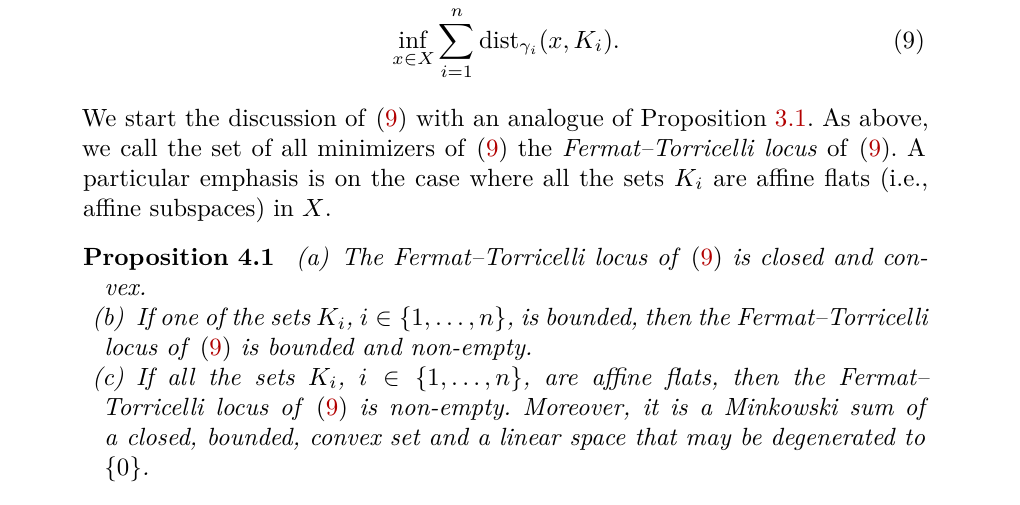
\includegraphics[width=0.98\linewidth]{figures/finite_affine_flat_statement_crop.png}
\end{center}

We give a full negative answer to the natural infinite-dimensional extension
of this statement, already for two closed affine flats and the ordinary
Hilbert norm.  We also determine exactly when the two-flat conclusion does
survive.

\section{Definitions and proof intuition}

For a nonempty subset $C$ of a real Hilbert space $\Hsp$, write
\[
 d(x,C)=\inf_{c\in C}\|x-c\|.
\]
For two target sets $A,B$, their minsum objective and locus are
\[
 F(x)=d(x,A)+d(x,B),\qquad \Argmin F.
\]
A closed affine flat has the form $a+U$, where $U$ is a closed linear
subspace.

\subsection*{Proof Intuition}

The finite-dimensional proof can force a minimizing sequence to converge
because sums of linear subspaces are closed.  Infinite-dimensional Hilbert
spaces have a precise new obstruction: two closed subspaces can have a
nonclosed algebraic sum.  For $A=a+U$ and $B=b+V$, finding a nearest pair is
exactly the problem of best-approximating $b-a$ by $U+V$.  The orthogonal
projection onto $\overline{U+V}$ always exists, but it need not lie in $U+V$.
That single missing membership is equivalent to an empty minsum locus.

For the explicit example, take the graph of the compact diagonal operator
$D(x)_n=x_n/n$.  Its range is dense and nonclosed.  The vector
$y=(1/n)$ is square summable but has only the formal preimage $(1,1,\ldots)$,
which is not in $\ell^2$.  Adding one orthogonal real coordinate makes the
unattained distance strictly positive, namely one.

\section{Exact theorem for two affine flats}

\begin{theorem}[Two-flat criterion and locus formula]\label{thm:criterion}
Let $\Hsp$ be a real Hilbert space, let $A=a+U$ and $B=b+V$ be nonempty
closed affine flats, and put
\[
 w=b-a,\qquad L=U+V,\qquad P=P_{\overline L}.
\]
Then:
\begin{enumerate}[label=\textup{(\roman*)}]
\item
\[
 \inf_{x\in\Hsp}\bigl(d(x,A)+d(x,B)\bigr)
 =\dist(A,B)=\dist(w,L)=\|(I-P)w\|.
\]
\item The minsum locus is nonempty if and only if $Pw\in L$.
\item Whenever $Pw\in L$, the entire locus is
\[
 \Argmin F
 =\bigcup\bigl\{[p,q]:p\in A,\ q\in B,\
                 \|p-q\|=\dist(A,B)\bigr\}.
\]
\item More generally, for $\alpha,\beta>0$,
\[
 \inf_x\{\alpha d(x,A)+\beta d(x,B)\}
 =\min\{\alpha,\beta\}\dist(A,B),
\]
and this weighted infimum is attained if and only if $Pw\in L$.
If $\alpha=\beta$, the locus is the union above.  If $\alpha<\beta$, it is
the set of endpoints in $B$ of nearest pairs; if $\beta<\alpha$, it is the
corresponding endpoint set in $A$.
\end{enumerate}
\end{theorem}

\begin{proof}
For every $x\in\Hsp$, the triangle inequality gives
\[
 \dist(A,B)\le d(x,A)+d(x,B).
\]
Conversely, evaluating at points of $A$ and then taking the infimum gives
\[
 \inf_x F(x)\le \inf_{p\in A}d(p,B)=\dist(A,B),
\]
so equality holds.

Suppose first that $F$ has a minimizer $x$.  Closed affine flats are closed
convex sets, hence have metric projections.  Put $p=P_Ax$ and $q=P_Bx$.
Then
\[
 \dist(A,B)\le\|p-q\|
 \le\|p-x\|+\|x-q\|=F(x)=\dist(A,B).
\]
Thus $(p,q)$ is a nearest pair.  Conversely, if $(p,q)$ is a nearest pair
and $x=(1-t)p+tq$, $0\le t\le1$, then
\[
 F(x)\le\|x-p\|+\|x-q\|=\|p-q\|=\dist(A,B),
\]
so every point of $[p,q]$ minimizes $F$.  Equality in the Hilbert-space
triangle inequality in the previous display forces any minimizer $x$ to lie
on the segment joining its projections $p$ and $q$.  This proves both the
attainment equivalence and the locus formula.

Differences of points of $A$ and $B$ range over
\[
 (a-b)+(U+V),
\]
because $V=-V$.  Hence
\[
 \dist(A,B)=\dist(w,L)=\dist(w,\overline L)=\|(I-P)w\|.
\]
The unique nearest point to $w$ in $\overline L$ is $Pw$.  Therefore the
distance to the algebraic sum $L$ is attained exactly when $Pw\in L$.
Together with the nearest-pair equivalence, this proves (i)--(iii).

Finally let $r=d(x,A)$, $s=d(x,B)$, and $d=\dist(A,B)$.  Since $r+s\ge d$,
\[
 \alpha r+\beta s\ge\min\{\alpha,\beta\}(r+s)
 \ge\min\{\alpha,\beta\}d.
\]
The reverse inequality follows by taking points in $B$ when $\alpha\le\beta$
(or in $A$ when $\beta\le\alpha$), so that the distance with the larger
coefficient vanishes.  If the
coefficients are unequal, equality also forces the distance to the
higher-weight flat to vanish; if they are equal, it forces $r+s=d$.
The asserted weighted loci and the same attainment criterion follow.
\end{proof}

\section{A positive-distance counterexample}

\begin{theorem}[Empty locus for two Hilbert affine flats]\label{thm:example}
There exist two nonempty closed affine flats $A,B$ in a separable real Hilbert
space such that
\[
 \dist(A,B)=1,
 \qquad
 \inf_x\bigl(d(x,A)+d(x,B)\bigr)=1,
 \qquad
 \Argmin F=\varnothing.
\]
Consequently, Proposition~4.1(c) of the source does not extend to
infinite-dimensional Hilbert spaces.
\end{theorem}

\begin{proof}
Let
\[
 \Hsp=(\ell^2\oplus\ell^2)\oplus\mathbb R,
 \qquad (Dx)_n=\frac{x_n}{n},
 \qquad y=\left(\frac1n\right)_{n\ge1}.
\]
The bounded operator $D:\ell^2\to\ell^2$ has a closed graph.  Moreover,
$y\in\ell^2$ but $y\notin\ran D$: a solution of $Dx=y$ would have
$x_n=1$ for every $n$.

Define
\[
 A=\ell^2\oplus\{0\}\oplus\{0\},
 \qquad
 B=(0,y,1)+\{(x,Dx,0):x\in\ell^2\}.
\]
Both are closed affine flats.  Every vector joining a point of $A$ to a point
of $B$ has last coordinate one, so $\dist(A,B)\ge1$.

For $N\ge1$, let $x^{(N)}=(-1,\ldots,-1,0,0,\ldots)$, with $N$ entries
equal to $-1$, and put
\[
 a_N=(x^{(N)},0,0)\in A,
 \qquad
 b_N=(x^{(N)},Dx^{(N)}+y,1)\in B.
\]
Then
\[
 \|a_N-b_N\|^2=1+\sum_{n>N}\frac1{n^2}\longrightarrow1.
\]
Thus $\dist(A,B)=1$.  If a pair attained this distance, equality with the
last-coordinate lower bound would force all other difference coordinates to
vanish, in particular $Dx=-y$ for some $x\in\ell^2$.  Its only formal
solution has $x_n=-1$ for all $n$, which is not in $\ell^2$.  Hence no
nearest pair exists.  Theorem~\ref{thm:criterion} now gives the stated
infimum and the empty locus.
\end{proof}

\begin{corollary}[Sharp positive replacement]
For two closed affine flats $a+U$ and $b+V$, closedness of $U+V$ guarantees a
nonempty minsum locus for every displacement $b-a$.  This applies, in
particular, if either direction is finite-dimensional or finite-codimensional.
Conversely, every nonclosed sum supplies displacements for which the locus is
empty.
\end{corollary}

\begin{proof}
If $U+V$ is closed, then $P_{\overline{U+V}}(b-a)$ automatically belongs to
$U+V$, so Theorem~\ref{thm:criterion} applies.  If one direction is
finite-dimensional, its image in the quotient by the other direction is a
finite-dimensional, hence closed, subspace.  If one direction has finite
codimension, the same quotient is finite-dimensional.  In either case the
preimage $U+V$ is closed.  For the converse, choose
$w\in\overline{U+V}\setminus(U+V)$; then $P_{\overline{U+V}}w=w\notin U+V$.
\end{proof}

The example also embeds in every infinite-dimensional Hilbert space: place it
in a closed separable summand and add the orthogonal complement to both affine
directions.  The two distance functions then depend only on the separable
coordinate.

\section{A standard positive compactness replacement}

For context, reflexivity does recover the source's bounded-target conclusion,
even though Theorem~\ref{thm:example} shows that it cannot recover the
all-affine-flat conclusion.

\begin{proposition}
Let $X$ be a reflexive Banach space.  Let $K_1,\ldots,K_m$ be nonempty
norm-closed convex sets, and let $\gamma_i$ be continuous gauges satisfying
$\gamma_i(z)\ge c_i\|z\|$ for constants $c_i>0$.  If one $K_i$ is bounded,
then
\[
 x\longmapsto\sum_{i=1}^m\inf_{y\in K_i}\gamma_i(y-x)
\]
attains its minimum, and its minimizer set is bounded and weakly compact.
\end{proposition}

\begin{proof}
Each gauge-distance is convex and norm-continuous, hence weakly lower
semicontinuous.  If $K_j$ is contained in a norm ball of radius $R$, then
\[
 \inf_{y\in K_j}\gamma_j(y-x)
 \ge c_j\inf_{y\in K_j}\|y-x\|
 \ge c_j(\|x\|-R).
\]
Thus the objective is coercive.  A minimizing sequence is bounded, has a
weakly convergent subsequence by reflexivity, and weak lower semicontinuity
gives a minimizer.  The minimizer set is bounded and weakly closed, hence
weakly compact.
\end{proof}

\section{Verification, limitations, and novelty}

The script \texttt{code/verify\_affine\_flat\_counterexample.py} checks the
explicit formula
\[
 \|a_N-b_N\|=\sqrt{1+\sum_{n>N}n^{-2}}
\]
for nine truncation sizes through $N=4096$, confirms convergence to one, and
records that the finite-dimensional preimage norm is $\sqrt N$ and escapes to
infinity.  It prints \texttt{VERDICT: PASS}.  This computation is a sanity
check, not part of the proof.

The precise two-flat theorem and counterexample are complete.  They do not
settle the source's broader questions for arbitrary finite families, general
asymmetric gauges, uniqueness, affine dimension of loci, Hadamard spaces, or
manifolds.

A bounded search through 13 August 2026 used the exact source title and arXiv
id, source citations, and combinations of the terms
\emph{infinite-dimensional minsum}, \emph{Fermat--Torricelli locus affine
flats}, \emph{closed affine subspaces distance not attained}, and
\emph{nonclosed sum Fermat--Torricelli}.  It also checked the 2011
variational-analysis paper arXiv:1009.1594 and the 2023 paper titled
\emph{The Generalized Fermat--Torricelli Problem in Hilbert Spaces}.  The
search found the standard theory of nonclosed subspace sums and later
algorithmic Hilbert-space work, but no paper presenting this exact
counterexample or criterion as an answer to Section~6.  Novelty is therefore
plausible, not certified.

\paragraph{Human-review recommendation.}
Send to a functional analyst.  The main checks are the equivalence between
minsum attainment and nearest-pair attainment, the membership condition
$P_{\overline{U+V}}(b-a)\in U+V$, and the source-to-subproblem match.

\begin{thebibliography}{9}
\bibitem{JahnKupitzMartiniRichter}
T.~Jahn, Y.~S.~Kupitz, H.~Martini, and C.~Richter,
\emph{Minsum Location Extended to Gauges and to Convex Sets},
Journal of Optimization Theory and Applications \textbf{166} (2015),
711--746; arXiv:1410.3690; doi:10.1007/s10957-014-0692-6.
\end{thebibliography}

\end{document}
